\documentclass[border=2mm,varwidth]{standalone}

\usepackage{tikz}
\usepackage{xcolor}

\usepackage{amsmath}


% Style setup
\usepackage{caption}
\usepackage{subcaption}
\captionsetup{format=plain, font=footnotesize, labelformat=empty}
\usepackage{colortbl}
%

% Notation setup
\usepackage{physics} % Braket notation

% Add qi.svg logo
\usepackage{svg}
\usepackage[absolute,overlay]{textpos}

% Newline in cell
\usepackage{makecell}

\begin{document}


$\ket{\color{red}\mathbf{q_0}\color{black},\color{red}\mathbf{q_1}\color{black}|q_2|\color{red}\mathbf{q_3}\color{black},\color{red}\mathbf{q_4}\color{black},\color{red}\mathbf{q_5}\color{black}|q_6,q_7} \Rightarrow \ket{q_2|q_6,q_7|\color{red}\mathbf{q_0}\color{black},\color{red}\mathbf{q_1}\color{black}|\color{red}\mathbf{q_3}\color{black},\color{red}\mathbf{q_4}\color{black},\color{red}\mathbf{q_5}\color{black}} $

\vspace{2mm}

Kövi:

\vspace{2mm}

$\ket{\color{red}\mathbf{0}\color{black},\color{red}\mathbf{0}\color{black}|0|\color{red}\mathbf{0}\color{black},\color{red}\mathbf{0}\color{black},\color{red}\mathbf{0}\color{black}|0,0}$

\vspace{2mm}

$\ket{0|0,0|\color{red}\mathbf{0}\color{black},\color{red}\mathbf{0}\color{black}|\color{red}\mathbf{0}\color{black},\color{red}\mathbf{0}\color{black},\color{red}\mathbf{0}\color{black}}$

\vspace{2mm}

Kövi:

\vspace{2mm}


$\ket{\color{red}\mathbf{0}\color{black},\color{red}\mathbf{0}\color{black}|1|\color{red}\mathbf{1}\color{black},\color{red}\mathbf{0}\color{black},\color{red}\mathbf{1}\color{black}|1,0}$

\vspace{2mm}

$\ket{1|1,0|\color{red}\mathbf{0}\color{black},\color{red}\mathbf{0}\color{black}|\color{red}\mathbf{1}\color{black},\color{red}\mathbf{0}\color{black},\color{red}\mathbf{1}\color{black}}$

\vspace{2mm}

Kövi:

\vspace{2mm}

$\ket{\color{red}\mathbf{0}\color{black},\color{red}\mathbf{1}\color{black}|1|\color{red}\mathbf{0}\color{black},\color{red}\mathbf{1}\color{black},\color{red}\mathbf{0}\color{black}|1,0}$

\vspace{2mm}

$\ket{1|1,0|\color{red}\mathbf{0}\color{black},\color{red}\mathbf{1}\color{black}|\color{red}\mathbf{0}\color{black},\color{red}\mathbf{1}\color{black},\color{red}\mathbf{0}\color{black}}$

\vspace{2mm}

Kövi:

\vspace{2mm}

$\ket{\color{red}\mathbf{1}\color{black},\color{red}\mathbf{0}\color{black}|0|\color{red}\mathbf{1}\color{black},\color{red}\mathbf{1}\color{black},\color{red}\mathbf{0}\color{black}|0,1}$

\vspace{2mm}

$\ket{0|0,1|\color{red}\mathbf{1}\color{black},\color{red}\mathbf{0}\color{black}|\color{red}\mathbf{1}\color{black},\color{red}\mathbf{1}\color{black},\color{red}\mathbf{0}\color{black}}$


\vspace{2mm}

Kövi:

\vspace{2mm}

$\ket{\color{red}\mathbf{1}\color{black},\color{red}\mathbf{0}\color{black}|0|\color{red}\mathbf{1}\color{black},\color{red}\mathbf{1}\color{black},\color{red}\mathbf{1}\color{black}|0,0}$

\vspace{2mm}

$\ket{0|0,0|\color{red}\mathbf{1}\color{black},\color{red}\mathbf{0}\color{black}|\color{red}\mathbf{1}\color{black},\color{red}\mathbf{1}\color{black},\color{red}\mathbf{1}\color{black}}$

\vspace{2mm}

Kövi:

\vspace{2mm}

$\ket{\color{red}\mathbf{1}\color{black},\color{red}\mathbf{1}\color{black}|1|\color{red}\mathbf{1}\color{black},\color{red}\mathbf{1}\color{black},\color{red}\mathbf{1}\color{black}|1,1}$

\vspace{2mm}

$\ket{1|1,1|\color{red}\mathbf{1}\color{black},\color{red}\mathbf{1}\color{black}|\color{red}\mathbf{1}\color{black},\color{red}\mathbf{1}\color{black},\color{red}\mathbf{1}\color{black}}$


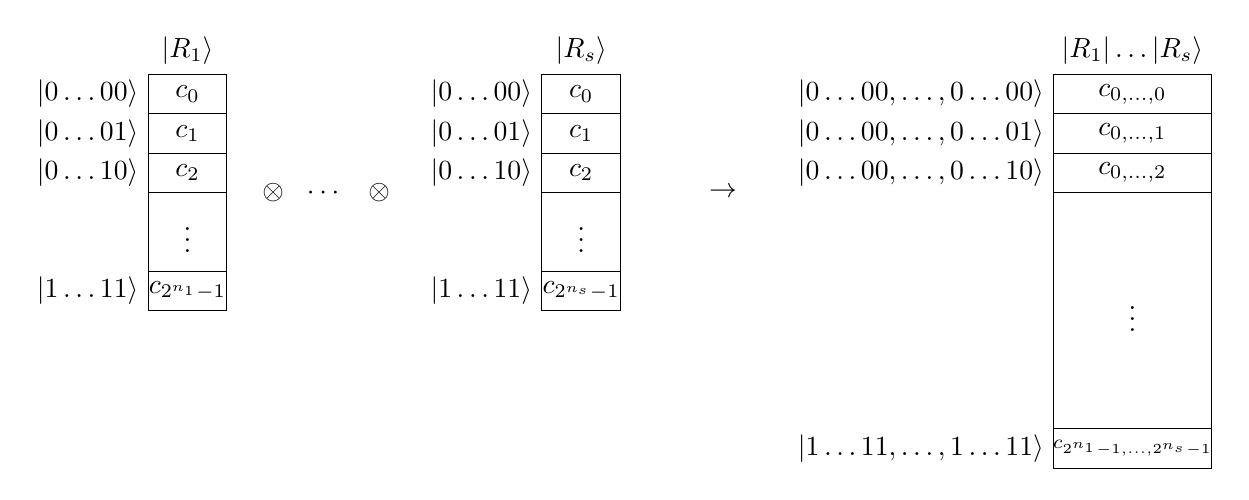
\begin{tikzpicture}

  \def\start{0}
  \def\w{1}
  \def\h{0.5}
  
  \node[anchor=south] at (\start+0.5*\w, \h) {$\ket{R_1}$};
  
  \draw (\start,0) rectangle (\start+\w,\h);
  \node[anchor=east] at (\start,0.5*\h) {$\ket{0\dots{}00}$};
  \node[align=center] at (\start+0.5*\w,0.5*\h) {$c_0$};
  
  \draw (\start,-1*\h) rectangle (\start+\w,0*\h);
  \node[anchor=east] at (\start, -1*\h + 0.5*\h) {$\ket{0\dots{}01}$};
  \node[align=center] at (\start + 0.5*\w, -1*\h + 0.5*\h) {$c_1$};
  
  \draw (\start,-2*\h) rectangle (\start+\w,-1*\h);
  \node[anchor=east] at (\start, -2*\h + 0.5*\h) {$\ket{0\dots{}10}$};
  \node[align=center] at (\start + 0.5*\w, -2*\h + 0.5*\h) {$c_2$};
  
  \draw (\start,-4*\h) rectangle (\start + \w,-2*\h);
  \node[align=center] at (\start + 0.5*\w, -4*\h + \h) {$\vdots{}$};
  
  \draw (\start,-5*\h) rectangle (\start + \w,-4*\h);
  \node[anchor=east] at (\start, -5*\h + 0.5*\h) {$\ket{1\dots{}11}$};
  \node[align=center] at (\start + 0.5*\w, -5*\h + 0.5*\h) {$c_{2^{n_1}-1}$};
  
  % Dots
  
  
  \node[align=center] at (2.3, -2*\h) {$\otimes{}~~\cdots{}~~\otimes{}$};
  
  % Masodik
  
  \def\start{5}
  
  \node[anchor=south] at (\start+0.5*\w, \h) {$\ket{R_s}$};
  
  \draw (\start,0) rectangle (\start+\w,\h);
  \node[anchor=east] at (\start,0.5*\h) {$\ket{0\dots{}00}$};
  \node[align=center] at (\start+0.5*\w,0.5*\h) {$c_0$};
  
  \draw (\start,-1*\h) rectangle (\start+\w,0*\h);
  \node[anchor=east] at (\start, -1*\h + 0.5*\h) {$\ket{0\dots{}01}$};
  \node[align=center] at (\start + 0.5*\w, -1*\h + 0.5*\h) {$c_1$};
  
  \draw (\start,-2*\h) rectangle (\start+\w,-1*\h);
  \node[anchor=east] at (\start, -2*\h + 0.5*\h) {$\ket{0\dots{}10}$};
  \node[align=center] at (\start + 0.5*\w, -2*\h + 0.5*\h) {$c_2$};
  
  \draw (\start,-4*\h) rectangle (\start + \w,-2*\h);
  \node[align=center] at (\start + 0.5*\w, -4*\h + \h) {$\vdots{}$};
  
  \draw (\start,-5*\h) rectangle (\start + \w,-4*\h);
  \node[anchor=east] at (\start, -5*\h + 0.5*\h) {$\ket{1\dots{}11}$};
  \node[align=center] at (\start + 0.5*\w, -5*\h + 0.5*\h) {$c_{2^{n_s}-1}$};
  
  % Rightarrow
  
  \node[align=center] at (7.3, -2*\h) {$\rightarrow$};
  
  % Uccso osszes
  
  
  \def\start{11.5}
  \def\w{2}
  
  \node[anchor=south] at (\start+0.5*\w, \h) {$\ket{R_1|\dots{}|R_s}$};
  
  \draw (\start,0) rectangle (\start+\w,\h);
  \node[anchor=east] at (\start,0.5*\h) {$\ket{0\dots{}00,\dots{},0\dots{}00}$};
  \node[align=center] at (\start+0.5*\w,0.5*\h) {$c_{0,\dots{},0}$};
  
  \draw (\start,-1*\h) rectangle (\start+\w,0*\h);
  \node[anchor=east] at (\start, -1*\h + 0.5*\h) {$\ket{0\dots{}00,\dots{},0\dots{}01}$};
  \node[align=center] at (\start + 0.5*\w, -1*\h + 0.5*\h) {$c_{0,\dots{},1}$};
  
  \draw (\start,-2*\h) rectangle (\start+\w,-1*\h);
  \node[anchor=east] at (\start, -2*\h + 0.5*\h) {$\ket{0\dots{}00,\dots{},0\dots{}10}$};
  \node[align=center] at (\start + 0.5*\w, -2*\h + 0.5*\h) {$c_{0,\dots{},2}$};
  
  \draw (\start,-8*\h) rectangle (\start + \w,-2*\h);
  \node[align=center] at (\start + 0.5*\w, -6*\h + \h) {$\vdots{}$};
  
  \draw (\start,-9*\h) rectangle (\start + \w,-8*\h);
  \node[anchor=east] at (\start, -9*\h + 0.5*\h)  {$\ket{1\dots{}11,\dots{},1\dots{}11}$};
  \node[align=center] at (\start + 0.5*\w, -9*\h + 0.5*\h) {\scriptsize$c_{2^{n_1}-1,\dots{}, 2^{n_s}-1}$};
  
  \end{tikzpicture}

% \def\layersep{2.5cm}
% \begin{tikzpicture}[shorten >=1pt,->,draw=black!50, node distance=\layersep,
%     %transform canvas={scale=1.5} <----- Comment out
% ]
%     \tikzstyle{every pin edge}=[<-,shorten <=1pt]
%     \tikzstyle{neuron}=[circle,fill=black!25,minimum size=17pt,inner sep=0pt]
%     \tikzstyle{input neuron}=[neuron, fill=green!50];
%     \tikzstyle{output neuron}=[neuron, fill=red!50];
%     \tikzstyle{hidden neuron}=[neuron, fill=blue!50];
%     \tikzstyle{hidden2 neuron}=[neuron, fill=blue!50];
%     \tikzstyle{annot} = [text width=4em, text centered]

% % Draw the input layer nodes
%     \foreach \name / \y in {1,...,4}
%     % This is the same as writing \foreach \name / \y in {1/1,2/2,3/3,4/4}
%         \node[input neuron, pin=left:Input \#\y] (I-\name) at (0,-\y) {};

% % Draw the hidden layer nodes
%     \foreach \name / \y in {1,...,5}
%         \path[yshift=0.5cm]
%             node[hidden neuron] (H-\name) at (\layersep,-\y cm) {};

%  % Draw the hidden layer nodes
%     \foreach \name / \y in {1,...,5}
%         \path[yshift=0.5cm]
%             node[hidden2 neuron] (H2-\name) at (\layersep*2,-\y cm) {};

% % Draw the output layer nodes
%       \foreach \name / \y in {1,...,3}
%         \path[yshift=0.5cm]
%             node[output neuron,pin=right:Class \#\y] (O-\name) at (\layersep*3,-\y cm) {};

% % Connect every node in the input layer with every node in the
% % hidden layer.
%     \foreach \source in {1,...,4}
%         \foreach \dest in {1,...,5}
%             \path (I-\source) edge (H-\dest);

%  % Connect every node in the first hidden layer with every node in the
% % second hidden layer.
%     \foreach \source in {1,...,5}
%         \foreach \dest in {1,...,5}
%             \path (H-\source) edge (H2-\dest);

% % Connect every node in the hidden layer with the output layer
%     \foreach \source in {1,...,5}
%         \foreach \dest in {1,...,3}
%             \path (H2-\source) edge (O-\dest);

% % Annotate the layers
%     \node[annot,above of=H-1, node distance=1cm] (hl) {Hidden layer 1};
%     \node[annot,above of=H2-1, node distance=1cm] (hl) {Hidden layer 2};
%     \node[annot,right of=hl] {Output layer};
% \end{tikzpicture}
\end{document}